%Esta charla puede ser descargada en http://people.ubuntu.com/~naguilarg/charlas/Contribuir-Debian
%Autor: Norman GArcía Aguilar norman@risuep.net

\documentclass{beamer}
%\usepackage[latin1]{inputenc}
\usepackage[spanish]{babel}
\usepackage{graphicx}
\usetheme{Warsaw}
\title{Como contribuir al proyecto Debian}
\author[n0rman]{Norman Garc\'ia \\ \texttt{norman@riseup.net}}
\institute{Debian Nicaragua}
\date{Octubre 20, 2011}
\begin{document}

\begin{frame}
	\titlepage
\end{frame}

\begin{frame}{Contenido}
	\tableofcontents
\end{frame}


\section{Introducci\'on}

\begin{frame}
\frametitle{¿Qu\'e es Debian GNU/Linux?}
        \begin{center}
                 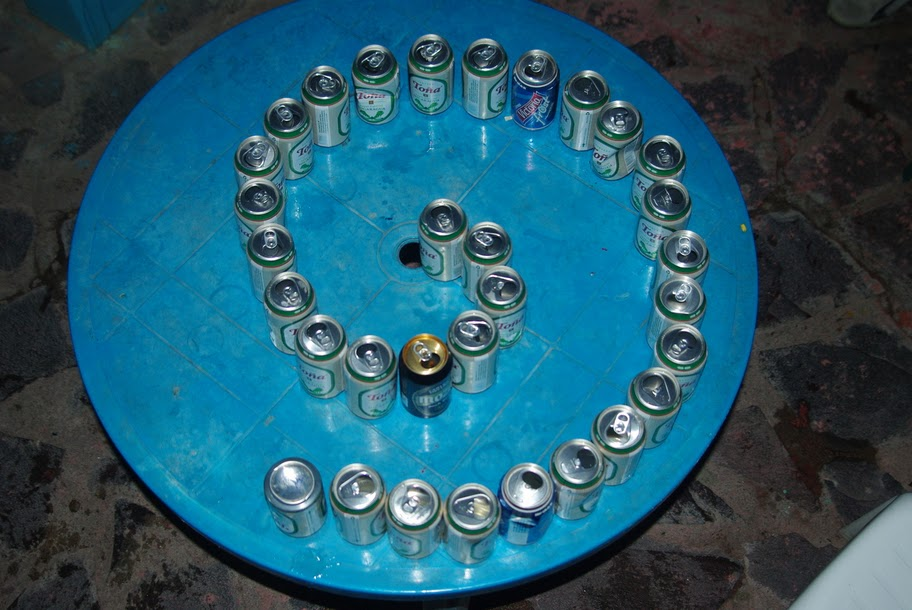
\includegraphics[scale=0.20]{../img/foto2950.jpg}
        \end{center}

        \pause

	Sistema operativo libre. El sistema operativo es el conjunto de programas b\'asicos y utilidades que 
        hacen que funcione su computadora. Debian utiliza el n\'ucleo Linux (el coraz\'on del sistema operativo), pero la mayor parte de las herramientas
        b\'asicas vienen del Proyecto GNU; de ah\'i el nombre GNU/Linux.
\end{frame}

\begin{frame}
\frametitle{¿Qu\'e es el proyecto Debian?}
        El Proyecto Debian es una asociaci\'on de personas que han hecho causa com\'un para crear un sistema operativo libre.
        \pause
        \begin{center}
                 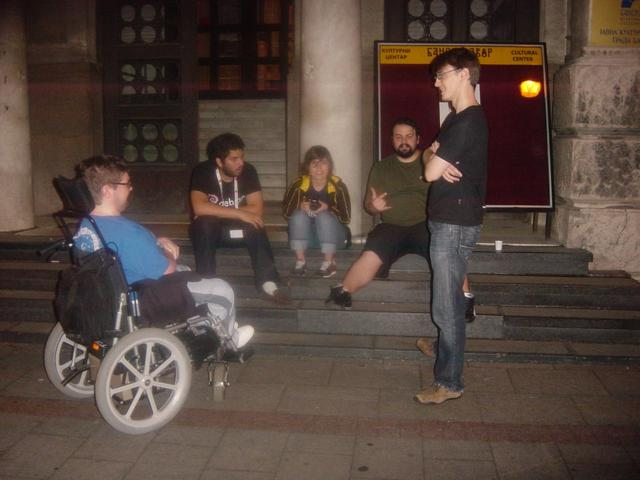
\includegraphics[scale=0.50]{../img/debconfproject.JPG}
        \end{center}
\end{frame}

\begin{frame}
\frametitle{Documentaci\'on}
\begin{itemize}
	\pause \item Constituci\'on del proyecto, Es un documento que describe los roles, derechos y deberes similar a la constituci\'on de un pau\'is norma la 
		mayor\'ia de aspectos relacionados a las leyes b\'asicas y de ella se derivan otros documentos.
	\pause \item DFSG o Gu\'ia del Software Libre para Debian, es un documento que define de manera clara que es lo que Debian considera Software Libre.
	\pause \item Social Contract - Contrato Social, es un documento que define los compromisos de Debian para con la sociedad.
\end{itemize}
\end{frame}


\section{Maneras de contribuir}
\begin{frame}
\frametitle{Usandolo}
    \begin{center}
             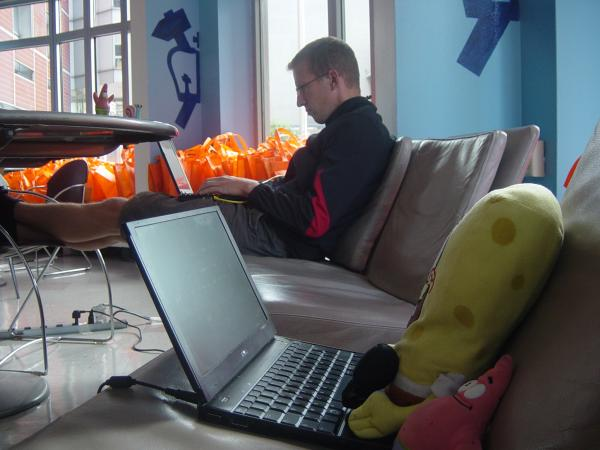
\includegraphics[scale=0.40]{../img/spongebob.JPG}
   \end{center}
\end{frame}

\begin{frame}
\frametitle{Usandolo}
       \begin{itemize}
                \pause \item Popularity Contest: \texttt{apt-get install popularity-contest}
                \pause \item \texttt{http://screenshots.debian.net}
        \end{itemize}
\end{frame}

\begin{frame}
\frametitle{Ayudando a otros}
       \begin{itemize}
                \pause \item Listas de correo \texttt{http://lists.debian.org/users.html}
		\pause \item Listas de correo \texttt{http://mail.debian.org.ni/mailman/listinfo}
                \pause \item irc \texttt{irc.debian.org}
                \pause \item foros \texttt{forums.debian.net}
                \pause \item wiki \texttt{wiki.debian.org}
        \end{itemize}
\end{frame}

\begin{frame}
\frametitle{Promoviendo Debian}
%buscar mejor foto
        \begin{center}
                 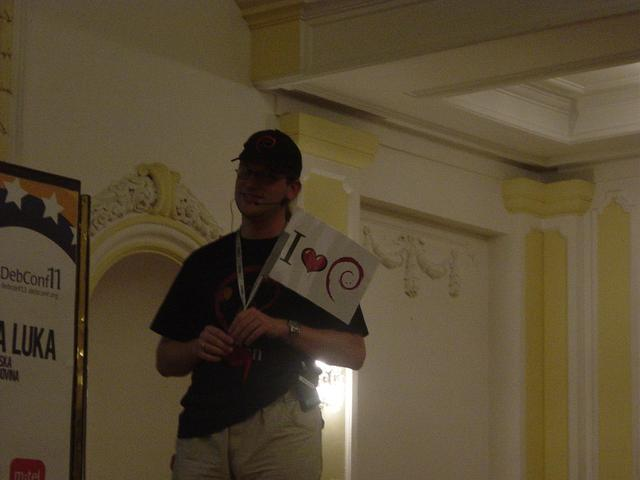
\includegraphics[scale=0.50]{../img/debianfanboy.JPG}
        \end{center}
\end{frame}

\begin{frame}
\frametitle{Promoviendo Debian}
        \begin{itemize}
                \pause \item Apoyando al equipo de publicidad. \texttt{http://lists.debian.org/debian-publicity/}
                \pause \item Hablar sobre Debian a otras personas. 
                \pause \item Representando a Debian.
        \end{itemize}

\end{frame}

\begin{frame}
\frametitle{Dando una charla}
        \begin{center}
                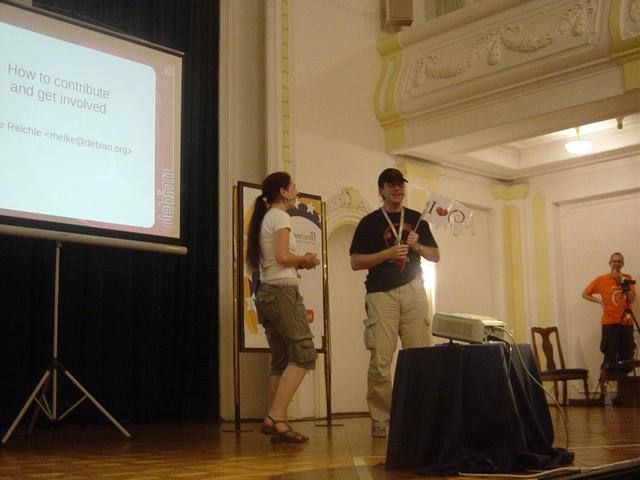
\includegraphics[scale=0.40]{../img/DSC00331.JPG}
        \end{center}

\end{frame}


\begin{frame}
\frametitle{Traduciendo}
        \begin{itemize}
                \pause \item Programas, documentaci\'on, sitio web.  \item \texttt{http://lists.debian.org/i18n.html}
		\pause \item Descripci\'on de paquetes. \texttt{http://ddtp.debian.net/ddtss}
		\pause \item Sitio web del equipo de traducci\'on. \texttt{www.debian.org/international/spanish/}
        \end{itemize}

\end{frame}

\begin{frame}
\frametitle{Traduciendo}
        \begin{center}
                 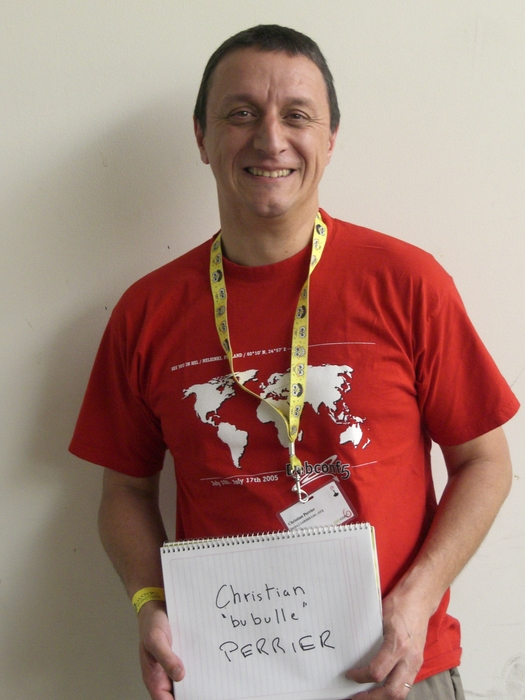
\includegraphics[scale=0.20]{../img/bubulle.jpg}
        \end{center}

\end{frame}

\begin{frame}

\frametitle{Siendo creativos}
        \begin{itemize}
                \pause \item Haciendo arte gr\'afico. Apoyando desde el equipo de arte.
                \pause \item Haciendo mejoras al sitio web.
                \pause \item Creando tutoriales.
        \end{itemize}

\end{frame}


\begin{frame}
\frametitle{Probando Debian}
        \begin{itemize}
                \pause \item Report\'a errores. \texttt{http://bugs.debian.org}
                \pause \item Reproduc\'i errores.
		\pause \item Prob\'a los nuevos lanzamientos.
        \end{itemize}

\end{frame}

\begin{frame}
\frametitle{Probando Debian}
        \begin{center}
                 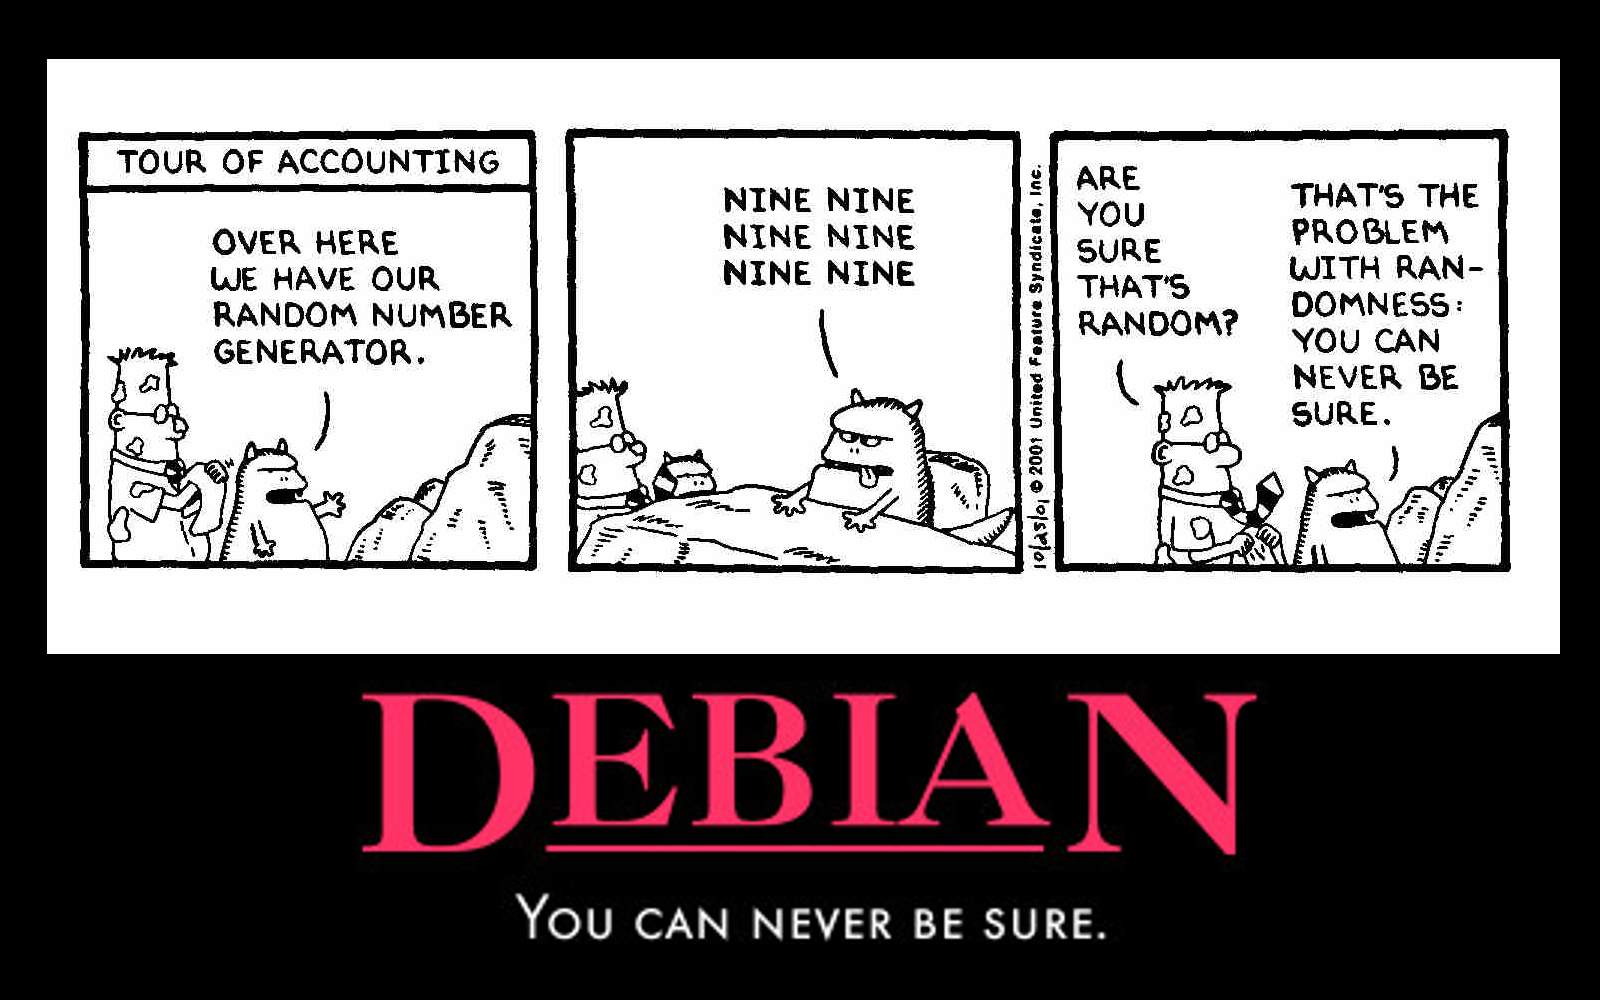
\includegraphics[scale=0.15]{../img/ReporteBug.png}
        \end{center}

\end{frame}


\begin{frame}
\frametitle{Eventos}
        \begin{itemize}
                 \pause \item Festivales de instalaci\'on.
		 \pause \item Bug squashing party (BPS).
		 \pause \item Apoyando en eventos.
        \end{itemize}
\end{frame}

\begin{frame}
\frametitle{Eventos}
        \begin{center}
                 
\includegraphics[scale=0.50]{../img/debconf_12_nicaragua.png}
        \end{center}
\end{frame}


\section{Razones para contribuir}

\begin{frame}
\frametitle{¿Qu\'e gano?}
             \begin{enumerate}
		\pause \item Aumentar mis conocimientos.
		\pause \item Convertirme en Debian Developer.
		\begin {itemize}
			\pause \item Derecho de voto.
			\pause \item Poder incorporar o hacer mejoras de cualquier software al sistema operativo Debian GNU/Linux.
			\pause \item Acceso a recursos del proyecto como servidores.
			\pause \item Tomar decisiones propias sobre su propio trabajo dentro del proyecto.
			\pause \item Postularse como Debian Project Leader.
			\pause \item \alert{NO ES NECESARIO SER MANTENER PAQUETES.}
		\end{itemize}
		\pause \item algunos DD que no mantienen paquetes.
		\begin{itemize}
			\pause \item Martin Baggage \texttt{brother-}: Mantiene traducciones a Sueco.
			\pause \item Francesa Ciceri \texttt{MadameZou}: Mantiene traducciones a Italiano, el sitio web y apoya al equipo de publicidad.
			\pause \item Matt Zimmerman: Se encarga de relaciones con distribuciones derivadas de Debian.
		\end{itemize}
	     \end{enumerate}
\end{frame}

\begin{frame}
\frametitle{¿Qu\'e gano?}
	\begin{center}
                 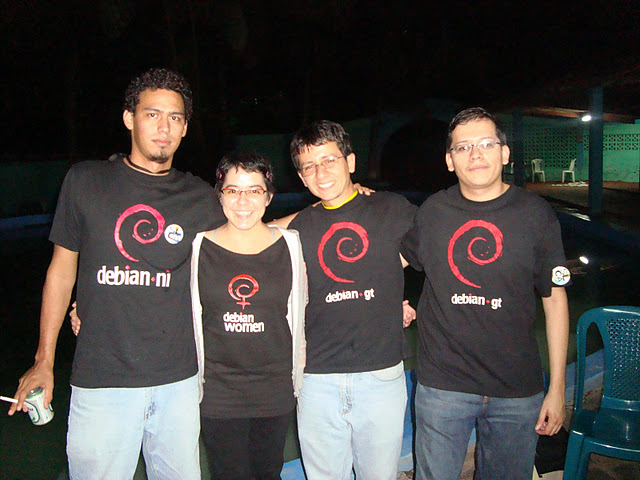
\includegraphics[scale=0.30]{../img/DSC03610.JPG}
	\end{center}
\end{frame}


\begin{frame}
\frametitle{¿Qu\'e gano?}
	\begin{center}
                 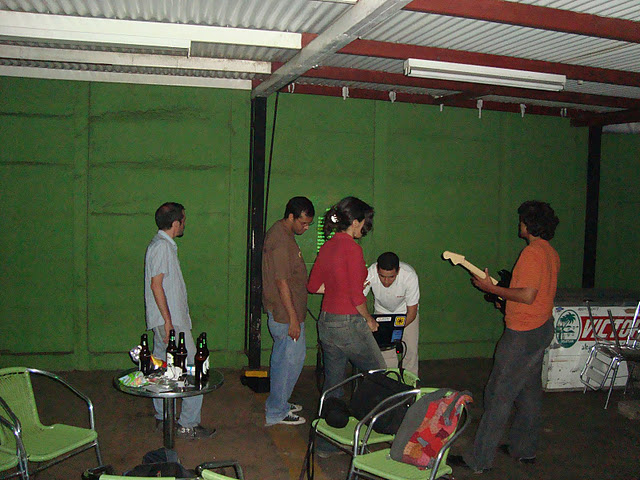
\includegraphics[scale=0.30]{../img/dsc04738.jpg}
	\end{center}
\end{frame}
\section{Gracias}


\begin{frame} 
\frametitle{¿Qu\'e gano?}
                 
\includegraphics[scale=0.30]{../img/dc11photogroup.jpg}
\end{frame}


\section{Gracias}


\begin{frame}
\frametitle{FIN}
	\begin{enumerate}
		\pause \item Presentaci\'on: Como contribuir con Debian GNU/Linux
		\pause \item Presentaci\'on basada en
			\begin{itemize}
				\pause \item How to contribute and get involved por \texttt{Meike Reichle y Alexander Reichle-Schmehl}
%					Puede descargar en  https://penta.debconf.org/penta/file/event_attachment/177?filename=howto-contribute.pdf
				\pause \item Contribuir con Debian por \texttt{Josue Abarca}
%					Puede descargar en http://jmaslibre.org/talks/contribuir_con_debian.pdf
			\end{itemize}
		\pause \item Presentado por: Norman Garc\'ia  \texttt{norman@riseup.net}
		\pause \item Octubre 20, 2011
		\pause \item Licencia: Creative Commons Atribuci\'on-CompartirIgual 3.0 Unported (CC BY-SA 3.0)
	\end{enumerate}

	\begin{center}
  		 
\includegraphics[scale=0.20]{../img/cclogo.png}
	\end{center}

\end{frame}
\end{document}
